% !TeX program = xelatex
\documentclass[10pt]{beamer}

\usetheme{metropolis}

\usepackage{pgfplots}
\usepgfplotslibrary{fillbetween}
\usepackage{pgfopts}
\usepackage{amsmath}
\usepackage{structuralanalysis}
\usepackage{tikz}
\usepackage{tikz-3dplot}
\usepackage{chngcntr}
\usepackage{wasysym}
\usepackage{mathtools}
\usepackage{alphalph}
\usepackage{xcolor}
\usepackage[showdow=false, en-US]{datetime2}
\usepackage{hyperref}

\newcommand{\highlight}[1]{%
	\colorbox{red!50}{$\displaystyle#1$}}

\setcounter{lecture}{17}
\counterwithin{equation}{lecture}
\makeatletter
\def\user@resume{resume}
\def\user@intermezzo{intermezzo}
%
\newcounter{previousequation}
\newcounter{lastsubequation}
\newcounter{savedparentequation}
\setcounter{savedparentequation}{1}
% 
\renewenvironment{subequations}[1][]{%
	\def\user@decides{#1}%
	\setcounter{previousequation}{\value{equation}}%
	\ifx\user@decides\user@resume 
	\setcounter{equation}{\value{savedparentequation}}%
	\else  
	\ifx\user@decides\user@intermezzo
	\refstepcounter{equation}%
	\else
	\setcounter{lastsubequation}{0}%
	\refstepcounter{equation}%
	\fi\fi
	\protected@edef\theHparentequation{%
		\@ifundefined {theHequation}\theequation \theHequation}%
	\protected@edef\theparentequation{\theequation}%
	\setcounter{parentequation}{\value{equation}}%
	\ifx\user@decides\user@resume 
	\setcounter{equation}{\value{lastsubequation}}%
	\else
	\setcounter{equation}{0}%
	\fi
	\def\theequation  {\theparentequation  \alph{equation}}%
	\def\theHequation {\theHparentequation \alph{equation}}%
	\ignorespaces
}{%
%  \arabic{equation};\arabic{savedparentequation};\arabic{lastsubequation}
\ifx\user@decides\user@resume
\setcounter{lastsubequation}{\value{equation}}%
\setcounter{equation}{\value{previousequation}}%
\else
\ifx\user@decides\user@intermezzo
\setcounter{equation}{\value{parentequation}}%
\else
\setcounter{lastsubequation}{\value{equation}}%
\setcounter{savedparentequation}{\value{parentequation}}%
\setcounter{equation}{\value{parentequation}}%
\fi\fi
%  \arabic{equation};\arabic{savedparentequation};\arabic{lastsubequation}
\ignorespacesafterend
}
\makeatother
\title{AE 737 - Mechanics of Damage Tolerance}
\subtitle{Lecture \arabic{lecture}}
\date{Last Updated: \today\ at \DTMcurrenttime}
\author{Dr. Nicholas Smith}
\institute{Wichita State University, Department of Aerospace Engineering}
% \titlegraphic{\hfill\includegraphics[height=1.5cm]{logo/logo}}

\begin{document}

\maketitle
\begin{frame}{schedule}
	\begin{itemize}
		\item 29 Mar - Influence of notches on fatigue, Homework 7 assigned, Homework 6 due
		\item 31 Mar - Strain based fatigue, project abstract due
		\item 5 Apr - Crack Growth, Homework 7 due, Homework 8 assigned
		\item 7 Apr - Crack Growth
	\end{itemize}
\end{frame}

\begin{frame}
  \frametitle{outline}
  \setbeamertemplate{section in toc}[sections numbered]
  \tableofcontents[hideallsubsections]
\end{frame}

\section{fatigue review}

%Group problems
\begin{frame}{group 1}
	\begin{itemize}
		\item A part from AISI 4340 in a typical "block" undergoes 100,000 cycles with $\sigma_{min} = 0 \text{ ksi}$ and $\sigma_{max} = 100 \text{ ksi}$ and an additional 10 cycles with $\sigma_{min} = 50 \text{ ksi}$ and $\sigma_{max} = 200 \text{ ksi}$
		\item How many "blocks" can this part support before failure?
	\end{itemize}
\end{frame}

\begin{frame}{group 2}
	\begin{itemize}
		\item Use the S-N-P chart on p. 245 for 7075-T6 Aluminum
		\item What is the probability of failure for 30 ksi at $10^6$ cycles?
		\item To ensure that 99\% of parts do not fail, after how many cycles should a fully reversed load of 35 ksi be inspected?
		\item How many cycles could the same part sustain if only 50\% of parts are needed?
	\end{itemize}
\end{frame}

\begin{frame}{group 3}
	\begin{itemize}
		\item The fatigue limit for AISI 4142 steel is 58 ksi for completely reversed fatigue loads.
		\item What is the fatigue limit for fatigue loads with $\sigma_m = 10, 20, 30 \text{ ksi}$?
	\end{itemize}
\end{frame}

\begin{frame}{group 4}
	\begin{itemize}
		\item A material made of 2024-T4 Aluminum undergoes the following load cycle
		\begin{itemize}
			\item $\sigma_{x,min} = 10$, $\sigma_{x,max} = 50$
			\item $\sigma_{y,min} = -20$, $\sigma_{y,max} = 20$
			\item $\tau_{xy,min} = 0$, $\tau_{xy,max} = 30$
		\end{itemize}
		\item How many cycles can it support before failure?
	\end{itemize}
\end{frame}

\section{influence of notches}

\begin{frame}{notch effects}
	\begin{itemize}[<+->]
		\item In this discussion, we use "notch" to refer to any geometric feature that increases the local stress (such as holes, fillets, grooves, etc.)
		\item We discussed notches and stress concentration factors in terms of stress concentration factors
		\item In our fatigue notation, $\sigma_{max} = K_t S$
		\item This relates local stress to the average, nominal stress
		\item The stress intensity factor can be used to characterize the "strength" of a notch
	\end{itemize}
\end{frame}

\begin{frame}{notch effects}
	\begin{itemize}[<+->]
		\item We might expect the fatigue life of a notched specimen to be similar to a pristine specimen with $S_{a,pristine} = \sigma_{max,notched}$
		\item If we look at actual test data, however, this estimate would be overly conservative
		\item Even when the stress is adjusted for some fatigue notch factor, $k_f$, it is only valid at longer cycles ($N_f > 10^6$)
		\item[] \begin{equation}
		k_f = \frac{\sigma_{ar}}{S_{ar}}
		\end{equation}
		\item Notches will have different effects, largely depending on their radius.
		\item The maximum possible fatigue notch factor is $k_f = k_t$
	\end{itemize}
\end{frame}

\begin{frame}{notch effects}
	\begin{figure}
	\centering
	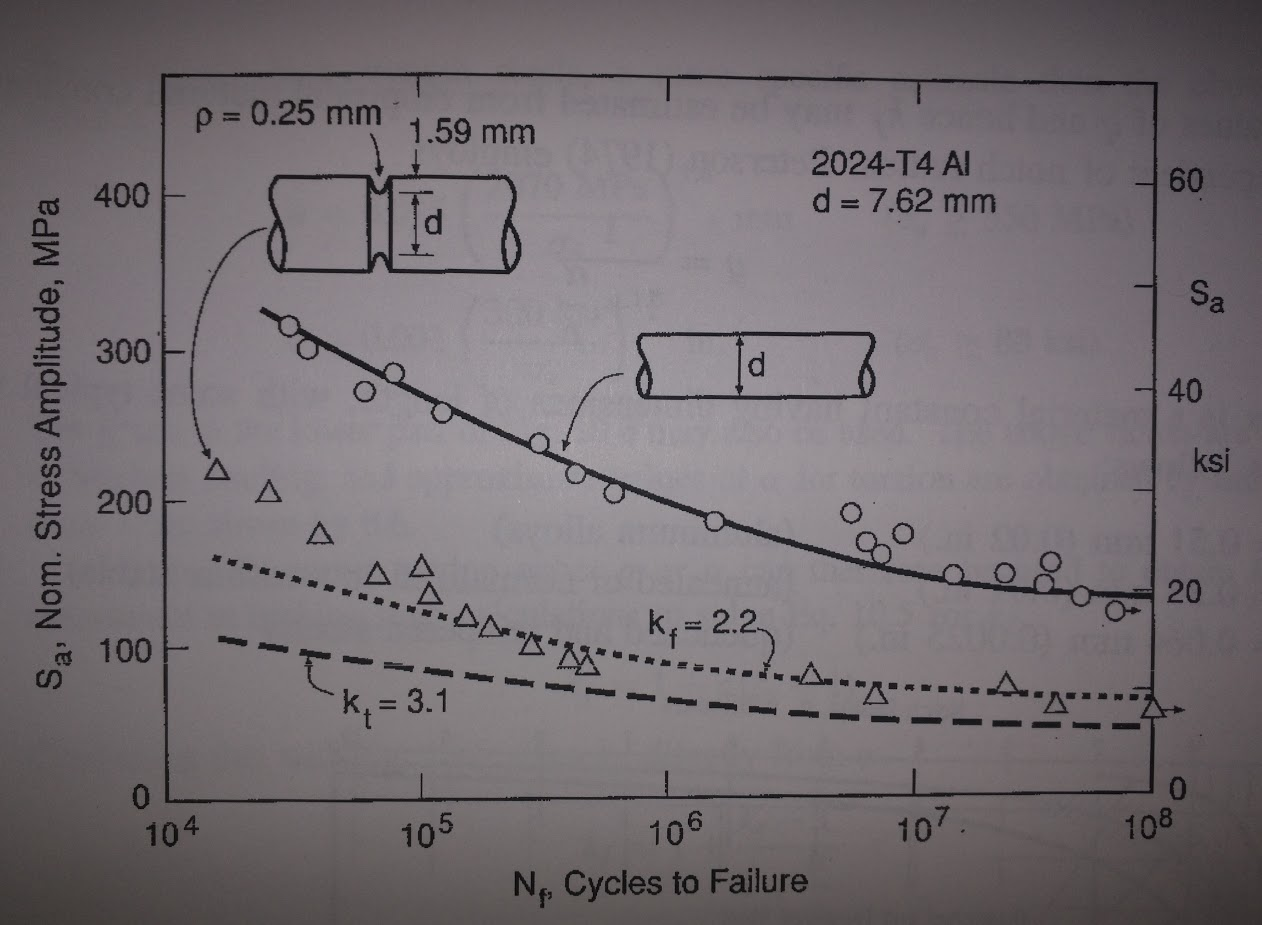
\includegraphics[width=0.7\linewidth]{../Figures/notch_effect}
	\label{fig:notch_effect}
	\end{figure}
\end{frame}

\begin{frame}{notch sensitivity factor}
	\begin{itemize}[<+->]
		\item To avoid generating fatigue data for every possible notch configuration, some empirical relationships have been developed
		\item A useful concept in these methods is the notch sensitivity factor
		\item[] \begin{equation}
		q = \frac{k_f - 1}{k_t -1}
		\end{equation}
		\item When $k_f = 1$, $q=0$, in which case the notch has no effect
		\item When $k_f = k_t$, $q=1$, in which case the notch has its maximum effect
	\end{itemize}
\end{frame}

\begin{frame}{peterson notch sensitivity}
	\begin{itemize}[<+->]
		\item Peterson developed the following relationship
		\item[] \begin{equation}
		q = \frac{1}{1+\frac{\alpha}{\rho}}
		\end{equation}
		\item Where $\rho$ is the radius of the notch
		\item $\alpha$ is a material property
		\item[]
		\begin{table}
			\caption{Table of $\alpha$ values for Peterson notch sensitivity equation}
		\begin{tabular}{ccc}
			Material & $\alpha$ (mm) & $\alpha$ (in) \\ 
			\hline Aluminum alloys & 0.51 & 0.02 \\ 
			 Annealed or low-carbon steels & 0.25 & 0.01 \\ 
			 Quenched and tempered steels & 0.064 & 0.0025 
		\end{tabular} 
		\end{table}
	\end{itemize}
\end{frame}

\begin{frame}{peterson notch sensitivy}
	\begin{itemize}[<+->]
		\item For high-strength steels, a more specific $\alpha$ estimate can be found
		\begin{align}
		\alpha &= 0.025 \left(\frac{2070 }{\sigma_u}\right)^{1.8} & \text{mm} & \qquad \sigma_u \ge 550 \text{ MPa}\\
		\alpha &= 0.001 \left(\frac{300 }{\sigma_u}\right)^{1.8} & \text{in} & \qquad \sigma_u \ge 80 \text{ ksi}
		\end{align}
		\item $\alpha$ predictions are valid for bending and axial fatigue
		\item For torsion fatigue, a good estimate can be found
		\item[] \begin{equation}
		\alpha_{torsion} = 0.6 \alpha
		\end{equation}
	\end{itemize}
\end{frame}

\begin{frame}{alternative notch sensitivity formulation}
	\begin{itemize}[<+->]
		\item An alternative formulation for $q$ was developed by Neuber
		\item[] \begin{equation}
		q = \frac{1}{1+\sqrt{\frac{\beta}{\rho}}}
		\end{equation}
		\item Where the material property $\beta$ for steels is given by
		\begin{align}
		\log \beta &= -\frac{\sigma_u - 134}{586} & \text{mm} & \qquad \sigma_u \le 1520 \text{ MPa}\\
		\log \beta &= -\frac{\sigma_u + 100}{85}& \text{in} & \qquad \sigma_u \le 220 \text{ ksi}
		\end{align}
		\item For aluminum use the chart MPa (ksi) and mm (in.)
		\begin{tabular}{c|ccc}
			$S_u$ & 150 (22) & 300 (43) & 600 (87) \\ 
			$\beta$ & 2 (0.08) & 0.6 (0.025) & 0.5 (0.015) \\ 
		\end{tabular} 
	\end{itemize}
\end{frame}

\begin{frame}{notch sensitivity factors}
	\begin{itemize}[<+->]
		\item While the above methods are useful, they should be regarded as estimates only
		\item Physical complexities are not fully modeled by these methods
		\item All of these have been developed for relatively "mild" notches
		\item For sharp notches, best results are found by treating the notch as a crack
	\end{itemize}
\end{frame}

\begin{frame}{example}
	\begin{itemize}
		\item Find the notch sensitivity factor for the following scenario
		\begin{align*}
		\rho &= 0.25 \text{ in.}\\
		\sigma_m &= 0 \text{ ksi}\\
		K_t &= 3.0\\
		\sigma_u &= 84 \text{ ksi}
		\end{align*}
	\end{itemize}
\end{frame}

\section{strain based fatigue}

\begin{frame}{strain based fatigue}
	\begin{itemize}[<+->]
		\item The strain based fatigue method uses local stresses and strains (instead of global, nominal values)
		\item The strain-based method gives greater detail, and validity at lower cycles
		\item It is still valid for high cycle fatigue
		\item Does not include crack growth analysis or fracture mechanics
	\end{itemize}
\end{frame}

\begin{frame}{strain life curve}
	\begin{itemize}[<+->]
		\item Similar to the S-N curves in stress-based fatigue analysis, we can plot the cyclic strain amplitude vs. number of cycles to failure
		\item This is most commonly done using axial test machines (instead of rotating bending tests)
		\item The test is run in strain control (not load control)
		\item Generally plotted on log-log scale
	\end{itemize}
\end{frame}

\begin{frame}{plastic and elastic strain}
	\begin{itemize}[<+->]
		\item We can separate the total strain into elastic and plastic components
		\item[] \begin{equation}
		\epsilon_a = \epsilon_{ea} + \epsilon_{pa}
		\end{equation}
	\end{itemize}
\end{frame}

\begin{frame}{plastic strain}
	\begin{figure}
	\centering
	\includegraphics[width=0.7\linewidth]{"../Figures/plastic_strain"}
	\label{fig:plasticstrain}
	\end{figure}
\end{frame}

\begin{frame}{hysteresis loops}
	\begin{figure}
	\centering
	\includegraphics[width=0.7\linewidth]{"../Figures/hysteresis_loops"}
	\label{fig:hysteresisloops}
\end{figure}
\end{frame}

\begin{frame}{cyclic stress strain curve}
	\begin{itemize}[<+->]
		\item While strain-life data will generally just report $\epsilon_a$ and $\epsilon_{pa}$, some will also tabulate a form for the cyclic stress-strain curve
		\item[] \begin{equation}
		\epsilon_a = \frac{\sigma_a}{E} + \left(\frac{\sigma_a}{H^\prime}\right)^{\frac{1}{n^\prime}}
		\end{equation}
	\end{itemize}
\end{frame}

\begin{frame}{plastic and elastic strain}
	\begin{itemize}[<+->]
		\item On strain life curves, the strain is often plotted three times per each experiment
		\item Once for total strain, once for plastic strain, and once for elastic strain
		\item Since plastic strain and elastic strain vary by the number of cycles, a hysteresis loop from half the fatigue life is generally used
		\item This is considered representative of stable behavior
	\end{itemize}
\end{frame}

\begin{frame}{experimental data}
	\begin{figure}
	\centering
	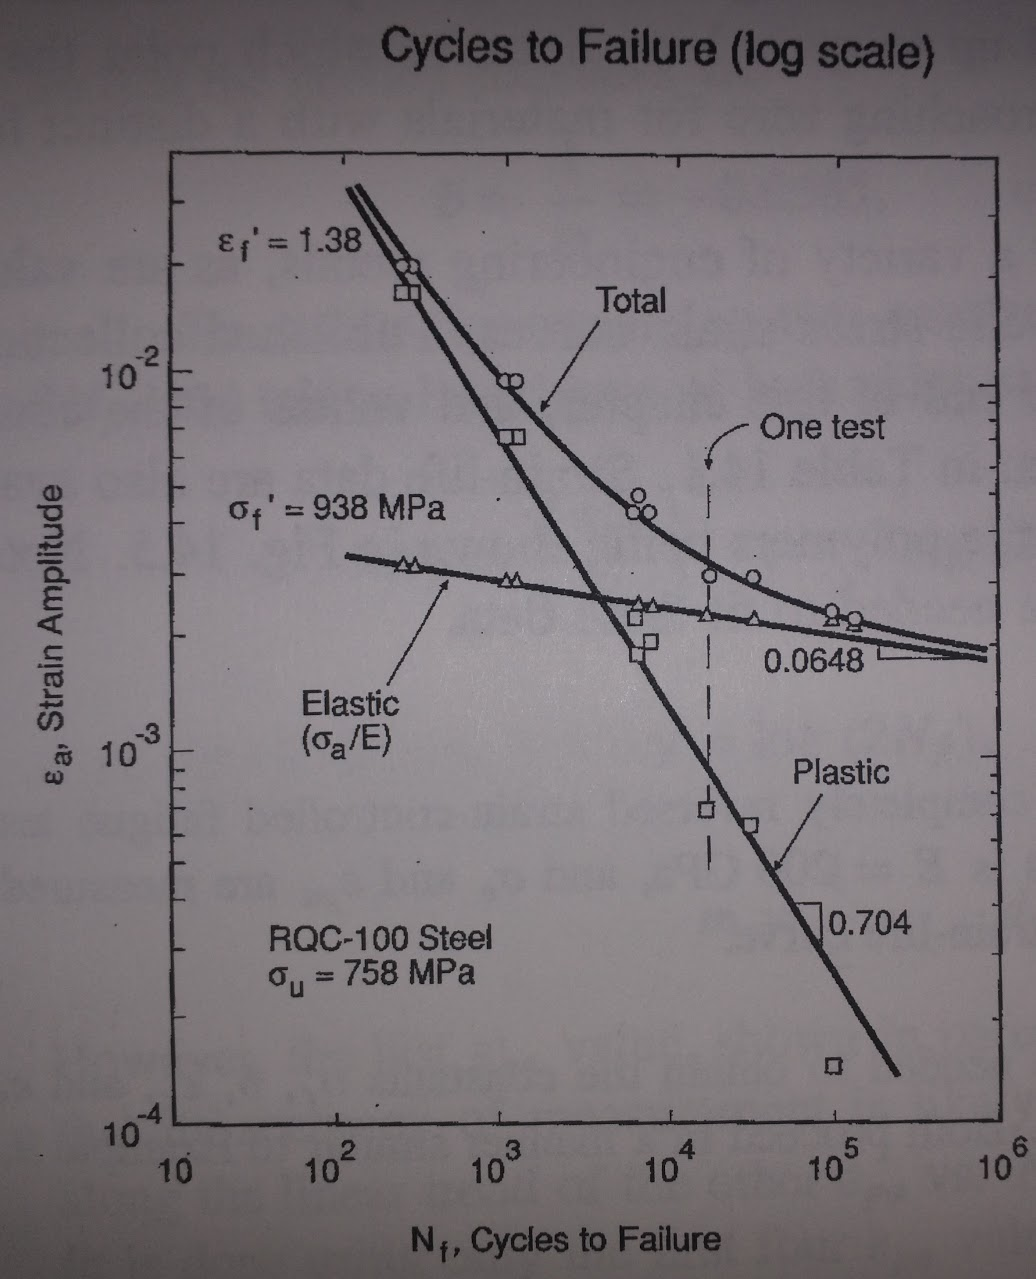
\includegraphics[width=0.5\linewidth]{../Figures/strain-life}
	\label{fig:strain-life}
	\end{figure}
\end{frame}

\begin{frame}{trends}
	\begin{figure}
	\centering
	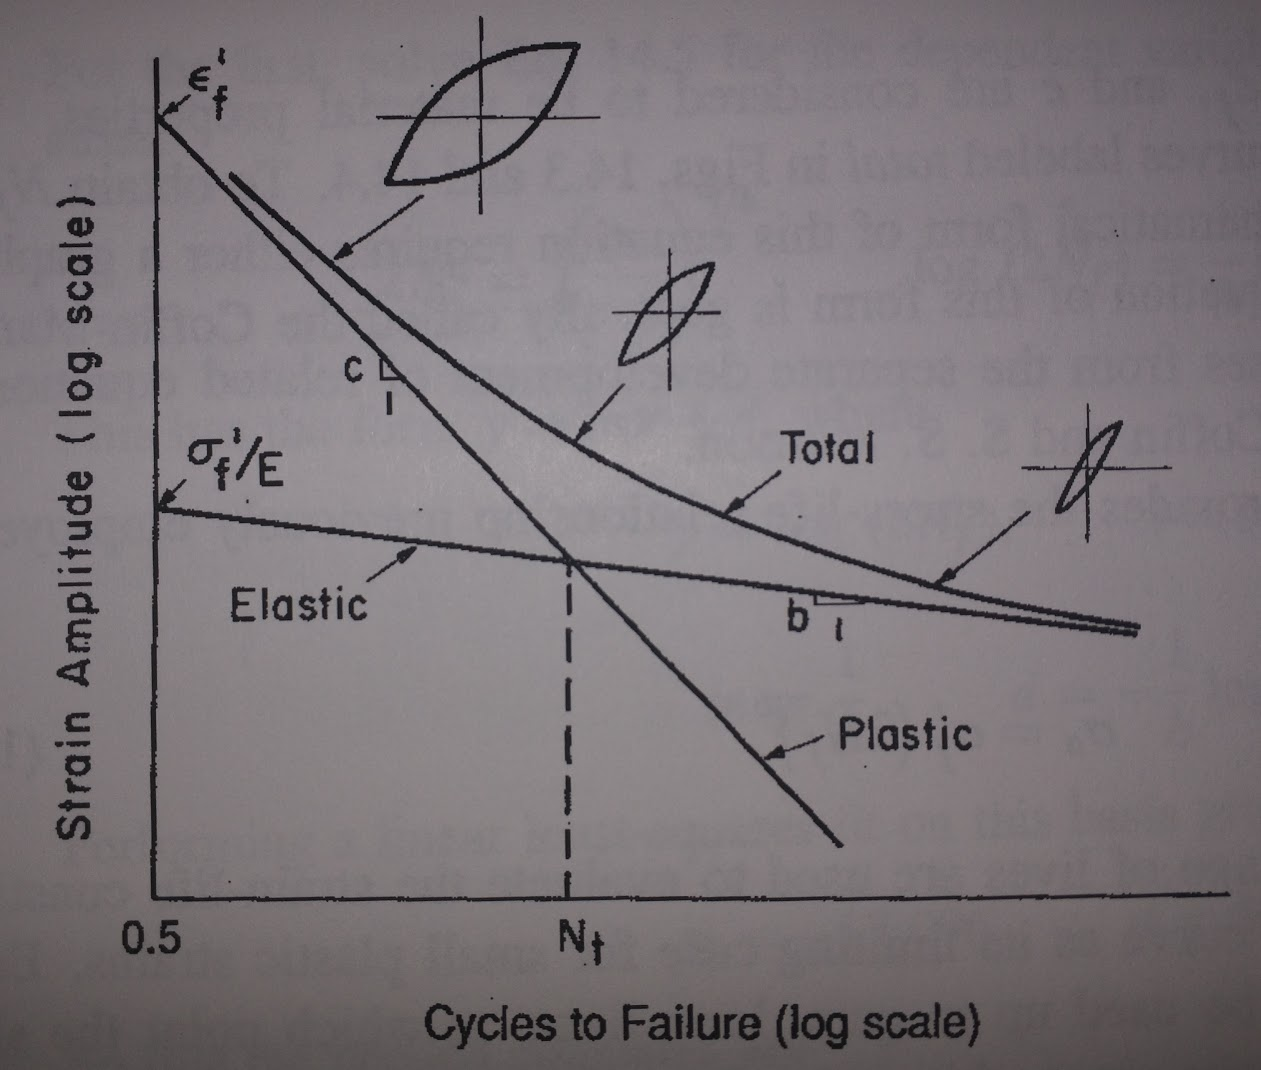
\includegraphics[width=0.7\linewidth]{../Figures/elastic-plastic}
	\label{fig:elastic-plastic}
	\end{figure}
\end{frame}

\begin{frame}{lines}
	\begin{itemize}[<+->]
		\item We notice that the data for elastic and plastic strains are represented by straight lines, in the log-log scale
		\item If we recall the form used for a straight line in log-log plots for S-N curves:
		\item[] \begin{equation}
		\sigma_a = \sigma_f^\prime (2N_f)^b
		\end{equation}
		\item We can convert this to find the elastic component of strain
		\item[] \begin{equation}
		\label{eq:elastic}
		\epsilon_{ea} = \frac{\sigma_f^\prime}{E} (2N_f)^b
		\end{equation}
	\end{itemize}
\end{frame}

\begin{frame}{lines}
	\begin{itemize}[<+->]
		\item We can use the same form with new constants for the plastic component of strain
		\item[]\begin{equation}
		\label{eq:plastic}
		\epsilon_{pa} = \epsilon_f^\prime (2 N_f)^c
		\end{equation}
		\item We can combine \ref{eq:elastic} with \ref{eq:plastic} to find the total strain-life curve
		\item[] \begin{equation}
		\epsilon_a = \frac{\sigma_f^\prime}{E} (2N_f)^b + \epsilon_f^\prime (2 N_f)^c
		\end{equation}
	\end{itemize}
\end{frame}

%TODO: second example
\begin{frame}{example}
	
\end{frame}

\end{document}
